\documentclass[12pt,a4paper]{article}
\newcommand{\AuthorName}
{نام و نام خانوادگی}
\newcommand{\AuthorSTID}
{شماره دانشجویی}

\usepackage{commons/course}
\usetikzlibrary{automata,positioning,arrows.meta}
\tikzset{
->,
>={Stealth[round]},
shorten >=1pt,
thick,
node distance=3cm,
every state/.style={thick, fill=gray!10},
initial text={$ $},
}

\lstset{
numbers=left, 
numberstyle=\small, 
numbersep=8pt, 
frame = single, 
language=Python,
framexleftmargin=15pt
}


%
%\let\ds\displaystyle
%\usepackage{arabtex}
%\usepackage[utf8]{inputenc}
%\usepackage[LFE,LAE]{fontenc}
%\usepackage[english,farsi]{babel}
%


\begin{document}



\سربرگ{تمرین سری اول}{اسکنر و گراف نحو}{99/7/22}



%نام و نام خانوادگی:پارسا نوری
%شماره دانشجویی: ۹۸۲۴۲۳۰۶۷


\مسئله{نام سؤال}

\پاسخ{}

الف)

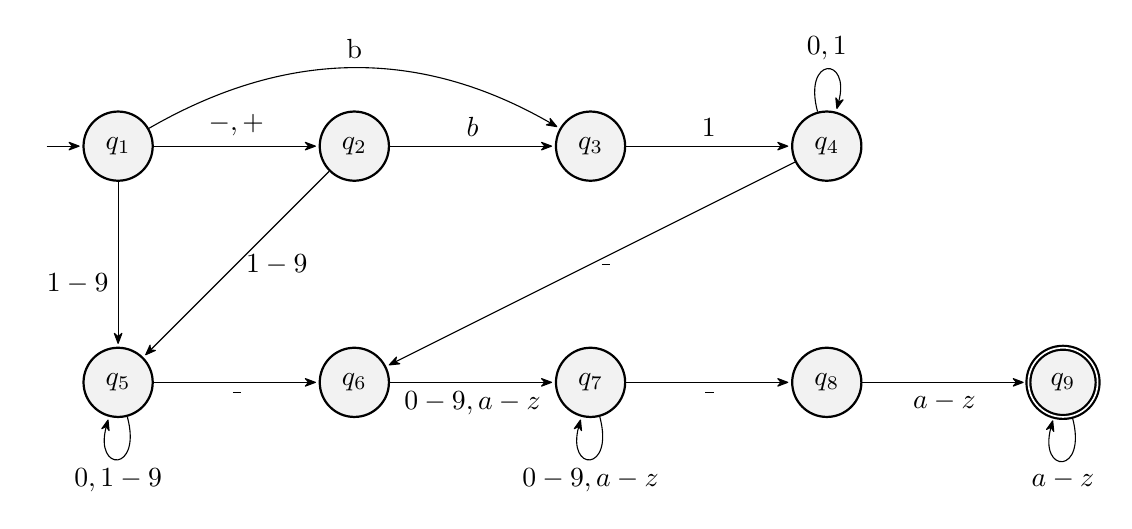
\begin{tikzpicture}
    \node[state,initial] (q1) {$q_1$};
    \node[state] (q2) [right of=q1] {$q_2$};
    \node[state] (q3) [right of=q2]{$q_3$};
    \node[state] (q4) [right of=q3]{$q_4$};
    \node[state] (q5) [below of=q1]{$q_5$};
    \node[state] (q6) [right of=q5]{$q_6$};
    \node[state] (q7) [right of=q6]{$q_7$};
    \node[state] (q8) [right of=q7]{$q_8$};
    \node[state,accepting] (q9) [right of=q8]{$q_9$};
    \draw (q1) edge[above] node{$-,+$} (q2);
    \draw (q1) edge[above] node[below left]{$1-9$} (q5);
    \draw (q1) edge[bend left, above] node{b} (q3);
    \draw (q2) edge[above] node{$b$} (q3);
    \draw (q2) edge[above] node[right]{$1-9$} (q5);
    \draw (q3) edge[above] node{$1$} (q4);
    \draw (q4) edge[loop above] node{$0,1$} (q4);
    \draw (q5) edge[loop below] node{$0,1-9$} (q5);
    %bakhsh e 1 ta inja too q4 o q5 e 
    \draw (q5) edge[above] node[below]{$\_$} (q6);
    \draw (q4) edge[above] node[right]{$\_$} (q6);
    %shoroo e bakhsh e 2
    \draw (q6) edge[above] node[below]{$0-9,a-z$} (q7);
    \draw (q7) edge[loop below] node[below]{$0-9,a-z$} (q7);
    %bakhsh e 2 alan too q7 ok shode
    \draw (q7) edge[above] node[below]{$\_$} (q8);
    \draw (q8) edge[above] node[below]{$a-z$} (q9);
    \draw (q9) edge[loop below] node[below]{$a-z$} (q9);
\end{tikzpicture}

ب)

\begin{latin}
    $((+|-)|\epsilon)((1-9)(0-9)^*|b1(0|1)^*)\_(a-z|0-9)^+\_(a-z)^+$
\end{latin}


%نام و نام خانوادگی:
%شماره دانشجویی: 
\مسئله{نام سؤال}

\پاسخ{}


%نام و نام خانوادگی:
%شماره دانشجویی: 
\مسئله{نام سؤال}


\پاسخ{}

الف) خیر کامپایلر از زبان سطح پایینتر به بالاتر نیز (همان دیکامپایل) و همچنین کامپایلر های زبان نرم افزار به سخت افزار هم داریم.

ب) در زبان های پویا کامپایل کردن سریع تر و عملکرد در زمان اجرا کند تر است. \newline
این برای آن است که کامپایلر بخشی از کارهایش را به زمان اجرا واگذاز میکند. پس کار های کمتری انجام داده و کند تر است. از طرفی در زمان اجرا این کار ها همچون link کردن باید انجام شود. که باعث میشود زمان اجرا کند تور شود.\newline
اگر بیایم برض کنیم که میخواهیم foo.bar() را اجرا کنیم باید ابتدا در \lr{Hash Table} دنبال foo بگردیم و بعد در \lr{Hash Table} مربوط به foo به دنبال آدرس bar(). این در حالی است که در رویکرد کامپایلری ما در جا آدرس foo و سپس در جا آدرس bar() را داریم. و دیگر نیازی به استفاده از \lr{Hash Table} نیست. از طرفی نیز در این رویکرد یک لایه باید برای ما خود بیاید و چیزی مثل بایت کد را به کد ماشین انجام دهد و این کار ممکن است تنها یک بار انجام نشود بلکه چند بار انجام شود(البته اگر بهینه سازی JIT انجام نشود که دور از ذهن نیست). این کارایی و سرعت را برای ما به شدت کاهش میدهد به قسمی که کل فرایند تبدیل کد سطح بالا تا کد ماشین ممکن خیلی خیلی و تا ۵۰ برابر کند ر از زبان های کامپایل شده انجام بشود. \newline

ج) 

\begin{latin}
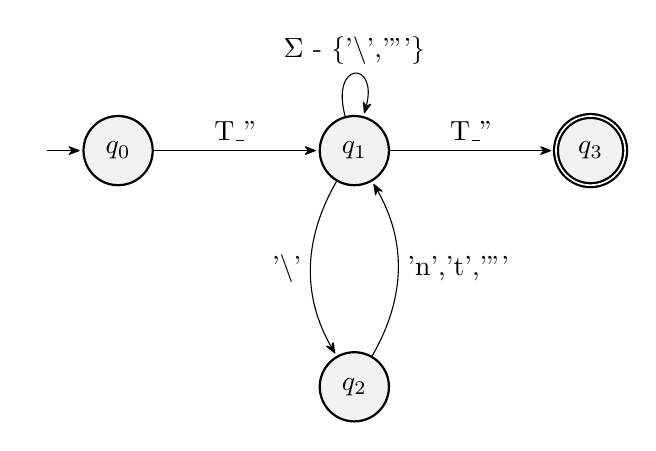
\begin{tikzpicture}

    \node[state,initial] (q0) {$q_0$};
    \node[state,right of=q0] (q1) {$q_1$};
    \node[state,below of=q1] (q2) {$q_2$};
    \node[state,right of=q1,accepting] (q3) {$q_3$};

    \draw (q0) edge[above] node{T\_"} (q1);
    \draw (q1) edge[bend right] node[left]{'\textbackslash'} (q2);
    \draw (q2) edge[bend right] node[right]{'n','t','"'} (q1);
    \draw (q1) edge[loop above] node{$\Sigma$ - \{'\textbackslash','"'\}} (q1);
    \draw (q1) edge[above] node{T\_"} (q3);

\end{tikzpicture}
\end{latin}


%نام و نام خانوادگی:
%شماره دانشجویی: 
\مسئله{نام سؤال}

\پاسخ{}

\begin{latin}
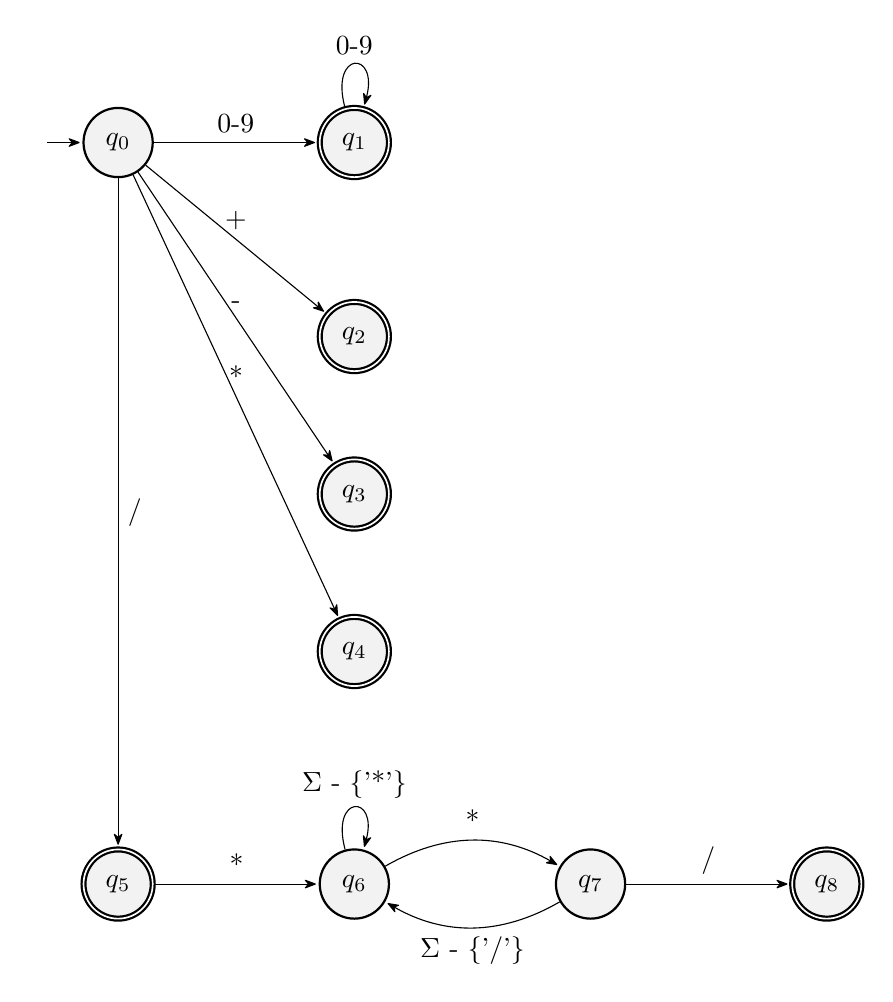
\begin{tikzpicture}
    \node[state, initial] (q0) {$q_0$};
    \node[state,right of=q0,accepting] (q1) {$q_1$};
    \node[state,right of=q0,below=2cm,accepting] (q2) {$q_2$};
    \node[state,right of=q0,below=4cm,accepting] (q3) {$q_3$};
    \node[state,right of=q0,below=6cm,accepting] (q4) {$q_4$};
    \node[state,below=8.5cm of q0,accepting] (q5) {$q_5$};
    \node[state,right of=q5] (q6) {$q_6$};
    \node[state,right of=q6] (q7) {$q_7$};
    \node[state,right of=q7,accepting] (q8) {$q_8$};
    
    \draw (q0) edge[above] node{0-9} (q1);
    \draw (q1) edge[loop above] node{0-9} (q1);
    \draw (q0) edge[above] node{+} (q2);
    \draw (q0) edge[above] node{-} (q3);
    \draw (q0) edge[above] node{*} (q4);
    \draw (q0) edge[right] node{/} (q5);
    \draw (q5) edge[above] node{*} (q6);
    \draw (q6) edge[loop above] node{$\Sigma$ - \{'*'\}} (q6);
    \draw (q6) edge[bend left] node[above]{*} (q7);
    \draw (q7) edge[bend left] node[below]{$\Sigma$ - \{'/'\}} (q6);
    \draw (q7) edge[above] node{/} (q8);

\end{tikzpicture}
\end{latin}


%نام و نام خانوادگی:
%شماره دانشجویی: 
\مسئله{نام سؤال}

\پاسخ{}

گراف به صورت زیر است:
در اینجا d بیانگر رقم است.
\begin{latin}
    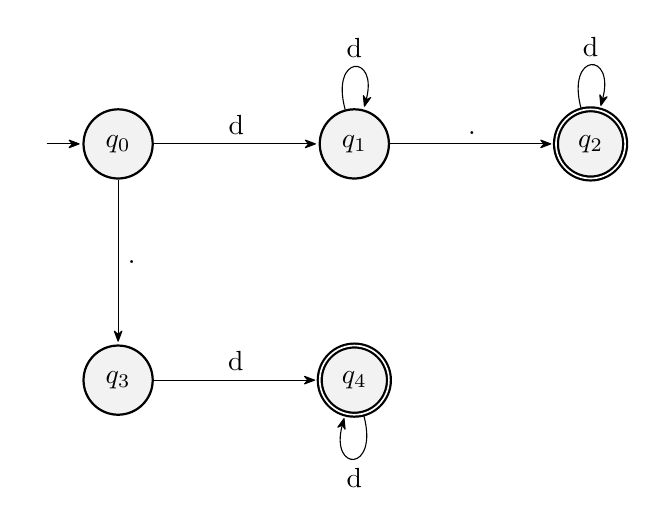
\begin{tikzpicture}
        \node[state,initial] (q0) {$q_0$};
        \node[state,right of=q0] (q1) {$q_1$};
        \node[state,right of=q1,accepting] (q2) {$q_2$};
        \node[state,below of=q0] (q3) {$q_3$};
        \node[state,right of=q3,accepting] (q4) {$q_4$};
        
        \draw (q0) edge[above] node{d} (q1);
        \draw (q1) edge[loop above] node{d} (q1);
        \draw (q1) edge[above] node{.} (q2);
        \draw (q2) edge[loop above] node{d} (q2);
        \draw (q0) edge[right] node{.} (q3);
        \draw (q3) edge[above] node{d} (q4);
        \draw (q4) edge[loop below] node{d} (q4);
    \end{tikzpicture}
\end{latin}
\newpage
کد به صورت زیر است:
\begin{latin}
    \begin{lstlisting}
#include <iostream>
#include <cctype>
using namespace std;

bool is_correct_float(const string& s){
    if (s == ".")
        return false;
    return all_of(s.begin(),s.end(),[] (const char c) -> bool {
        return isdigit(c) || c == '.';
    }) && any_of(s.begin(),s.end(),[] (const char c) -> bool {
        return c == '.';
    });
}
int main()
{
    string s = "2345678.";
    cout << (is_correct_float(s) ? "true" : "false") << endl;
    return 0;
}
    \end{lstlisting}
\end{latin}


%نام و نام خانوادگی:
%شماره دانشجویی: 
\مسئله{نام سؤال}

\پاسخ{}

%نام و نام خانوادگی:
%شماره دانشجویی: 
\مسئله{نام سؤال}

\پاسخ{}

\begin{latin}
    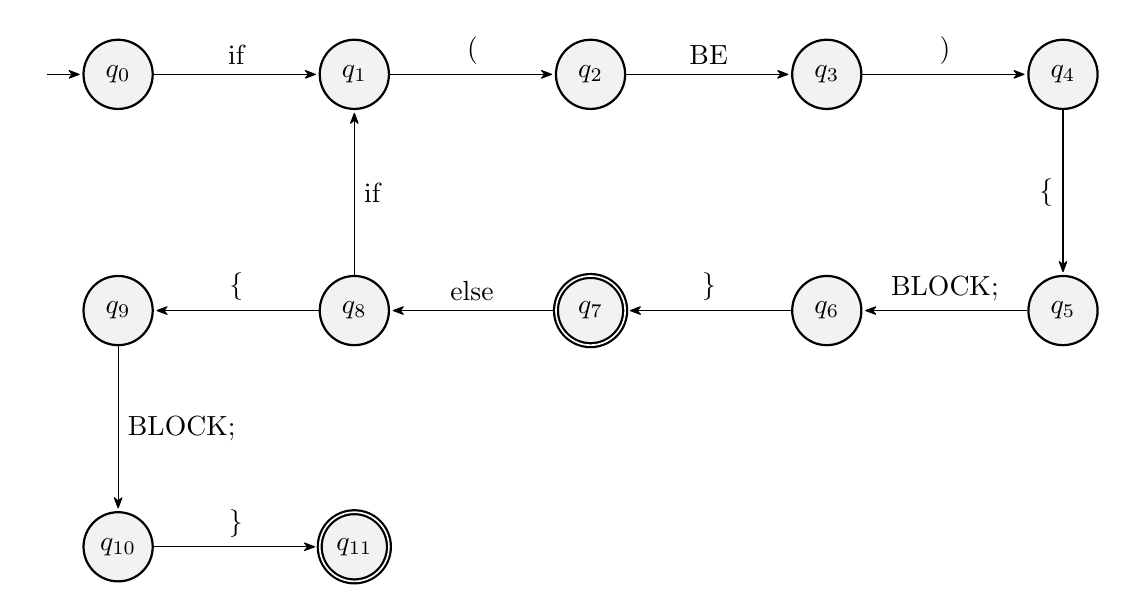
\begin{tikzpicture}
    
    \node[state,initial] (q0) {$q_0$};
    \node[state,right of=q0] (q1) {$q_1$};
    \node[state,right of=q1] (q2) {$q_2$};
    \node[state,right of=q2] (q3) {$q_3$};
    \node[state,right of=q3] (q4) {$q_4$};
    \node[state,below of=q4] (q5) {$q_5$};
    \node[state,left of=q5] (q6) {$q_6$};
    \node[state,left of=q6,accepting] (q7) {$q_7$};
    \node[state,left of=q7] (q8) {$q_8$};
    \node[state,left of=q8] (q9) {$q_9$};
    \node[state,below of=q9] (q10) {$q_{10}$};
    \node[state,right of=q10,accepting] (q11) {$q_{11}$};

    \draw (q0) edge[above] node{if} (q1);
    \draw (q1) edge[above] node{(} (q2);
    \draw (q2) edge[above] node{BE} (q3);
    \draw (q3) edge[above] node{)} (q4);
    \draw (q4) edge[left] node{\{} (q5);
    \draw (q5) edge[above] node{BLOCK;} (q6);
    \draw (q6) edge[above] node{\}} (q7);
    \draw (q7) edge[above] node{else} (q8);
    \draw (q8) edge[above] node{\{} (q9);
    \draw (q9) edge[right] node{BLOCK;} (q10);
    \draw (q10) edge[above] node{\}} (q11);
    \draw (q8) edge[right] node{if} (q1);

     \end{tikzpicture}
\end{latin}


%نام و نام خانوادگی:
%شماره دانشجویی: 
\مسئله{نام سؤال}

\پاسخ{}

الف) دیگر بین ضرب و جمع الویتی قائل نیستیم و هر کدام که زودتر بیاید آن را انجام می‌دهیم.

ب) 

\begin{latin}
    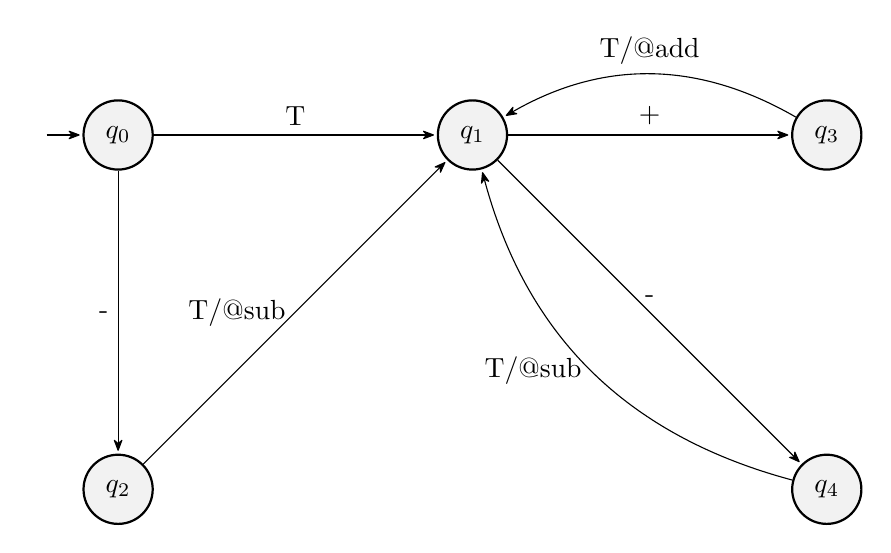
\begin{tikzpicture}[node distance=4.5cm]
        \node[state, initial] (q0) {$q_0$};
        \node[state, right of=q0] (q1) {$q_1$};
        \node[state, below of=q0] (q2) {$q_2$};
        \node[state, right of=q1] (q3) {$q_3$};
        \node[state, below of=q3] (q4) {$q_4$};
        
        \draw (q0) edge[above] node{T} (q1);
        \draw (q0) edge[left] node{-} (q2);
        \draw (q2) edge[left] node{T/@sub} (q1);
        \draw (q1) edge[above] node{+} (q3);
        \draw (q1) edge[above] node{-} (q4);
        \draw (q4) edge[bend left] node[left]{T/@sub} (q1);
        \draw (q3) edge[bend right] node[above]{T/@add} (q1);
        
    \end{tikzpicture}
\end{latin}


%نام و نام خانوادگی:
%شماره دانشجویی: 
\مسئله{نام سؤال}

\پاسخ{}

   
\end{document}

